\documentclass[12pt, a4paper]{article}

\usepackage{amssymb}
\usepackage{amsmath}
\usepackage{bm}
\usepackage{geometry}
\usepackage{graphicx}
\usepackage{adjustbox}
\usepackage[font=small,labelfont=bf]{caption}
\usepackage{tikz}
\usetikzlibrary{arrows,automata}
\usepackage[thinlines]{easytable}

\title{Rapport \'Evaluation de performances de r\'eseaux}
\author{Morgane Cadeau, Morgan Canas, Lucas Lafage, William Mateille, Raphael Sombstay}
\date{Novembre 2019}

\makeatletter         
\def\@maketitle{
\raggedright
\begin{center}
\vspace*{\fill}
{\Huge \bfseries \sffamily \@title }\\[4ex] 
{\Large  \@author}\\[4ex] 
\@date\\[8ex]
\includegraphics[width=10cm]{logo-enseeiht}
\vspace*{\fill}
\end{center}}
\makeatother

\begin{document}
\maketitle
\thispagestyle{empty}
\newpage
\tableofcontents
\setcounter{page}{1}

\newpage

\section*{Comparaison de files d'attente}
\includegraphics[width=\linewidth]{exercice1}
\captionof{figure}{Sch\'ema des diff\'erents syst\`emes}

\subsection*{Temps moyen de r\'eponse du syst\`eme 1}

\quad Calcul du nombre moyen de clients dans la file

\[\rho=\frac{\lambda}{2\mu}\]
\[E[L]=\frac{\rho}{1-\rho} \text{ donc}\]
\[E[L]=\frac{\lambda}{2\mu} * \frac{1}{1-\frac{\lambda}{2\mu}} = \frac{\lambda}{2\mu} * \frac{1}{\frac{2\mu-\lambda}{2\mu}}=\frac{\lambda}{2\mu}*\frac{2\mu}{2\mu-\lambda}\]
\boldmath\[E[L]=\frac{\lambda}{2\mu-\lambda}\]\unboldmath
\linebreak

\quad Calcul du temps moyen de r\'eponse du syst\`eme

\[E[R]=\frac{E[L]}{\lambda}\]
\[E[R]=\frac{\lambda}{2\mu-\lambda}*\frac{1}{\lambda}\]
\boldmath\[E[R]=\frac{1}{2\mu-\lambda}\]\unboldmath
\newpage
\subsection*{Temps moyen de r\'eponse du syst\`eme 2}
\medskip

\begin{center}
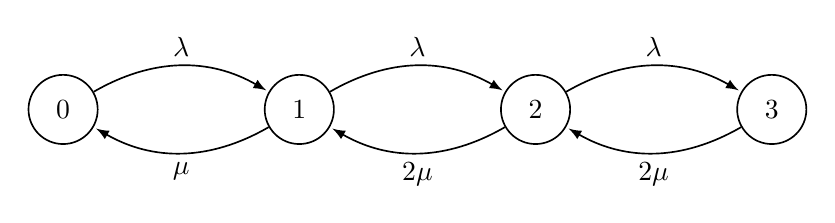
\begin{tikzpicture}[
            > = stealth, % arrow head style
            shorten > = 1pt, % don't touch arrow head to node
            auto,
            node distance = 3cm, % distance between nodes
            semithick % line style
        ]

	\node[state] (0) {$0$};
	\node[state] (1) [right of=0] {$1$};
	\node[state] (2) [right of=1] {$2$};
	\node[state] (3) [right of=2] {$3$};
	
	\draw[-latex,bend left] (0) edge node {$\lambda$} (1);
	\draw[-latex,bend left] (1) edge node {$\mu$} (0);
	\draw[-latex,bend left] (1) edge node {$\lambda$} (2);
	\draw[-latex,bend left] (2) edge node {$2\mu$} (1);
 	\draw[-latex,bend left] (2) edge node {$\lambda$} (3);
	\draw[-latex,bend left] (3) edge node {$2\mu$} (2);
   
\end{tikzpicture}
\captionof{figure}{Cha\^ine de Markov du syst\`eme de 0 \`a 3 clients}
\end{center}
\medskip
On peut donc en d\'eduire la cha\^ine de Markov du syst\`eme pour $n$ clients :
\begin{center}
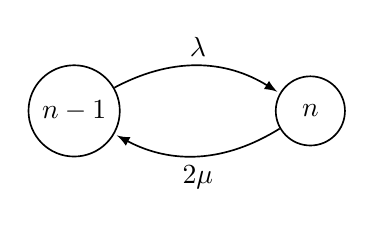
\begin{tikzpicture}[
            > = stealth, % arrow head style
            shorten > = 1pt, % don't touch arrow head to node
            auto,
            node distance = 3cm, % distance between nodes
            semithick % line style
        ]

	\node[state] (A) {$n-1$};
	\node[state] (B) [right of=A] {$n$};
	
 	\draw[-latex,bend left] (A) edge node {$\lambda$} (B);
	\draw[-latex,bend left] (B) edge node {$2\mu$} (A);
   
\end{tikzpicture}
\captionof{figure}{Cha\^ine de Markov du syst\`eme pour $n$ clients}
\end{center}

\bigskip
\quad Utilisation de la m\'ethode des coupes afin de d\'eterminer $\pi_{n}$ selon $\pi_{0}$

\begin{gather*}
\pi_{0}\lambda=\pi_{1}\mu \\
\bm{\pi_{1}=\frac{\lambda}{\mu}\pi_{0}} \\
2\mu\pi_{2}=\lambda\pi_{1}=\frac{\lambda^{2}}{\mu}\pi_{0} \\
\bm{\pi_{2}=\frac{\lambda^{2}}{2\mu^{2}}\pi_{0}} \\
2\mu\pi_{3}=\lambda\pi_{2}=\frac{\lambda^{3}}{2\mu^{2}}\pi_{0} \\
\bm{\pi_{3}=\frac{\lambda^{3}}{4\mu^{3}}\pi_{0}} \\
\text{On a donc }\pi_{n}=\frac{\lambda}{2\mu}\pi_{n-1} \\
\text{On en d\'eduit que }\bm{\pi_{n}=\frac{\lambda^{n}}{2^{n-1}\mu^{n}}\pi_{0}} \\
\text{Or }\rho=\frac{\lambda}{2\mu} \text{ donc } \bm{\pi_{n}=2\rho^{n}\pi_{0}} \\
\end{gather*}

\quad Calcul de $\pi_{0}$ gr\^ace \`a la somme des probabilit\'es

\begin{gather*}
\pi_{0}+\sum_{i=1}^{\infty} \pi_{i} = 1 \\
\pi_{0}=1-\sum_{i=1}^{\infty}\pi_{i} \\
\pi_{0}=1-\sum_{i=1}^{\infty}2\rho^{i}\pi_{0} \\
\pi_{0}=1-2\pi_{0} \sum_{i=1}^{\infty}\rho^{i} \\
\Rightarrow \pi_{0}=1-2\pi_{0}\rho\sum_{i=0}^{\infty}\rho^{i} \\
\pi_{0}=1-2\pi_{0}\rho\left(\frac{1}{1-\rho}\right) \text{ car } \sum_{i=0}^{\infty}\rho^{i}=\frac{1}{1-\rho}\\
\pi_{0}=1-\frac{2\rho}{1-\rho}\pi_{0} \\
\Rightarrow 1 = \pi_{0}+\frac{2\rho}{1-\rho}\pi_{0} \\
1=\pi_{0}\left(1+\frac{2\rho}{1-\rho}\right)=\frac{1-\rho+2\rho}{1-\rho}\pi_{0} \\
\Rightarrow \bm{\pi_{0}=\frac{1-\rho}{1+\rho}} \\
\end{gather*}

\quad La valeur de $\pi_{0}$ nous permet de d\'eduire $\pi_{n}$
\[\bm{\pi_{n}=2\rho^{n}\frac{1-\rho}{1+\rho}}\]

\newpage
\quad Calcul du nombre moyen de clients dans la file

\begin{gather*}
E[L]=\sum_{i=0}^{\infty}i\pi_{i} \\
E[L]=\sum_{i=0}^{\infty}i2\rho^{i}\frac{1-\rho}{1+\rho} \\
E[L]=2\left(\frac{1-\rho}{1+\rho}\right)\sum_{i=0}^{\infty}i\rho^{i} \\
\Rightarrow E[L]=2\left(\frac{1-\rho}{1+\rho}\right)\frac{\rho}{\left(1-\rho\right)^{2}} \text{ car } \sum_{i=0}^{\infty}i\rho^{i} = \frac{\rho}{\left(1-\rho\right)^{2}} \\
E[L]=\frac{2\rho}{\left(1+\rho\right)\left(1-\rho\right)} \\
\Rightarrow \bm{E[L]=\frac{2\rho}{1-\rho^{2}}}
\end{gather*}

\quad Calcul du temps moyen de r\'eponses du syst\`eme 2
\begin{gather*}
E[R]=\frac{E[L]}{\lambda} \\
E[R]=\frac{2\rho}{\lambda\left(1-\rho^{2}\right)} = \frac{2\lambda}{2\mu\lambda\left(1-\rho^{2}\right)} \\
\bm{E[R]=\frac{1}{\mu\left(1-\rho^{2}\right)}}
\end{gather*}

\newpage
\subsection*{Nombre moyen de passages d'un client et temps de réponse moyen dans chacune des 2 files du syst\`eme 3}

On peut appliquer le th\'eor\`eme de Jackson car toutes les hypoth\`eses sont respect\'ees
\begin{itemize}
\item Arriv\'ees selon un processus de poisson de d\'ebit $\lambda$
\item Chaque file a 1 seul serveur, un service exponentiel de param\`etre $\mu$, une capacit\'e infinie est est FIFO
\end{itemize}

\medskip
\quad Calcul de la charge $\rho$ 

\begin{gather*}
e_{1} = e_{2} = \frac{1}{2} \\
\lambda_{1} = \lambda_{2} = \frac{1}{2}\lambda \\
\rho_{1} = \rho_{2} = \frac{1}{2}\frac{\lambda}{\mu} = \bm{\frac{\lambda}{2\mu}}
\end{gather*}

\quad Calcul du nombre moyen de passages d'un client dans chacune des 2 files

\begin{gather*}
E[L_{i}] = \frac{\rho_{i}}{1-\rho_{i}} \text{ et on sait que } \rho_{1}=\rho_{2} \\
E[L_{1}] = E[L_{2}] = \frac{\frac{\lambda}{2\mu}}{1-\frac{\lambda}{2\mu}} = \frac{\frac{\lambda}{2\mu}}{\frac{2\mu - \lambda}{2\mu}} \\
E[L_{1}] = E[L_{2}] = \frac{\lambda}{2\mu}\times\frac{2\mu}{2\mu - \lambda} \\
\bm{E[L_{1}] = E[L_{2}] = \frac{\lambda}{2\mu - \lambda}}
\end{gather*}

\quad Calcul du temps moyen de r\'eponse du syst\`eme

\begin{gather*}
E[R_{i}] = \frac{E[L_{i}]}{\lambda e_{i}} \text{ et on sait que } E[L_{1}] = E[L_{2}] \text{ et } e_{1}=e_{2} \\
E[R_{1}]=\frac{E[L_{1}]}{\lambda_{1}}=\frac{\lambda}{2\mu-\lambda}\times\frac{1}{\frac{1}{2}\lambda} \\
E[R_{1}]=\frac{2}{2\mu-\lambda} = \frac{1}{\mu-\frac{1}{2}\lambda}
\end{gather*}

\begin{gather*}
\text{Or } E[L_{1}]=E[L_{2}] \text{ et } \lambda_{1}=\lambda_{2} \text{ donc} \\
\bm{E[R_{1}]=E[R_{2}]=\frac{1}{\mu-\frac{1}{2}\lambda}} \\
E[R]=e_{1}E[R_{1}]+e_{2}E[R_{2} ]\\
E[R]=\frac{1}{2\left(\mu-\frac{1}{2}\lambda\right)}+\frac{1}{2\left(\mu-\frac{1}{2}\lambda\right)} \\
\bm{E[R]=\frac{2}{2\mu-\lambda}=\frac{1}{\mu-\frac{1}{2}\lambda}}
\end{gather*}
\bigskip

\subsection*{Classement des 3 syst\`emes en fonction de leurs performances respectives}

\bigskip

\begin{TAB}(r,1cm,1cm)[5pt]{|c|c|c|}{|c|c|c|c|}
	 & Temps moyen de r\'eponse & Temps de r\'eponse pour $\mu=1$ et $\lambda=1$ \\
	 Syst\`eme 1 & $\frac{1}{2\mu-\lambda}$ & 1 \\
	 Syst\`eme 2 & $\frac{1}{\mu\left(1-\rho^{2}\right)}$ & $\frac{4}{3}$ \\
	 Syst\`eme 3 & $\frac{1}{\mu-\frac{1}{2}\lambda}$ & 2 \\
\end{TAB}
\captionof{figure}{Tableau de comparaison des performances des 3 syst\`emes}

\bigskip
\quad Le syst\`eme 1 est le plus efficace car son temps de r\'eponse est plus faible pour la m\^eme valeur de $\mu$ et de $\lambda$ entre les 3 syst\`emes. \medskip

\quad Ce r\'esultat \'etait pr\'evisible car le syst\`eme 1 a un serveur 2 fois plus rapide que les autres syst\`emes. Ainsi, s'il n'y a qu'un client, ce syst\`eme est plus rapide que le syst\`eme 2.

\newpage
\subsection*{Performances si on a un syst\`eme 3 bis o\`u les clients se dirigent vers la file la moins remplie}
\quad Dans ce cas l\`a, le syst\`eme 3 bis serait plus performant que le syst\`eme 3 car le temps de r\'eponse serait inf\'erieur. Cependant, le syst\`eme 2 aurait tout de m\^eme un temps moyen de r\'eponse sup\'erieur \`a celui du syst\`eme 2. \medskip

\quad Le classement serait donc le suivant :
\begin{enumerate}
\item Syst\`eme 1
\item Syst\`eme 2
\item Syst\`eme 3 bis
\item Syst\`eme 4
\end{enumerate}

\newpage

\subsection*{Montrer que $N(t)=(N1(t),N2(t))$ est markovien et construire la cha\^ine de Markov pour des files inf\'erieures ou \'egales \`a 3}

\begin{center}
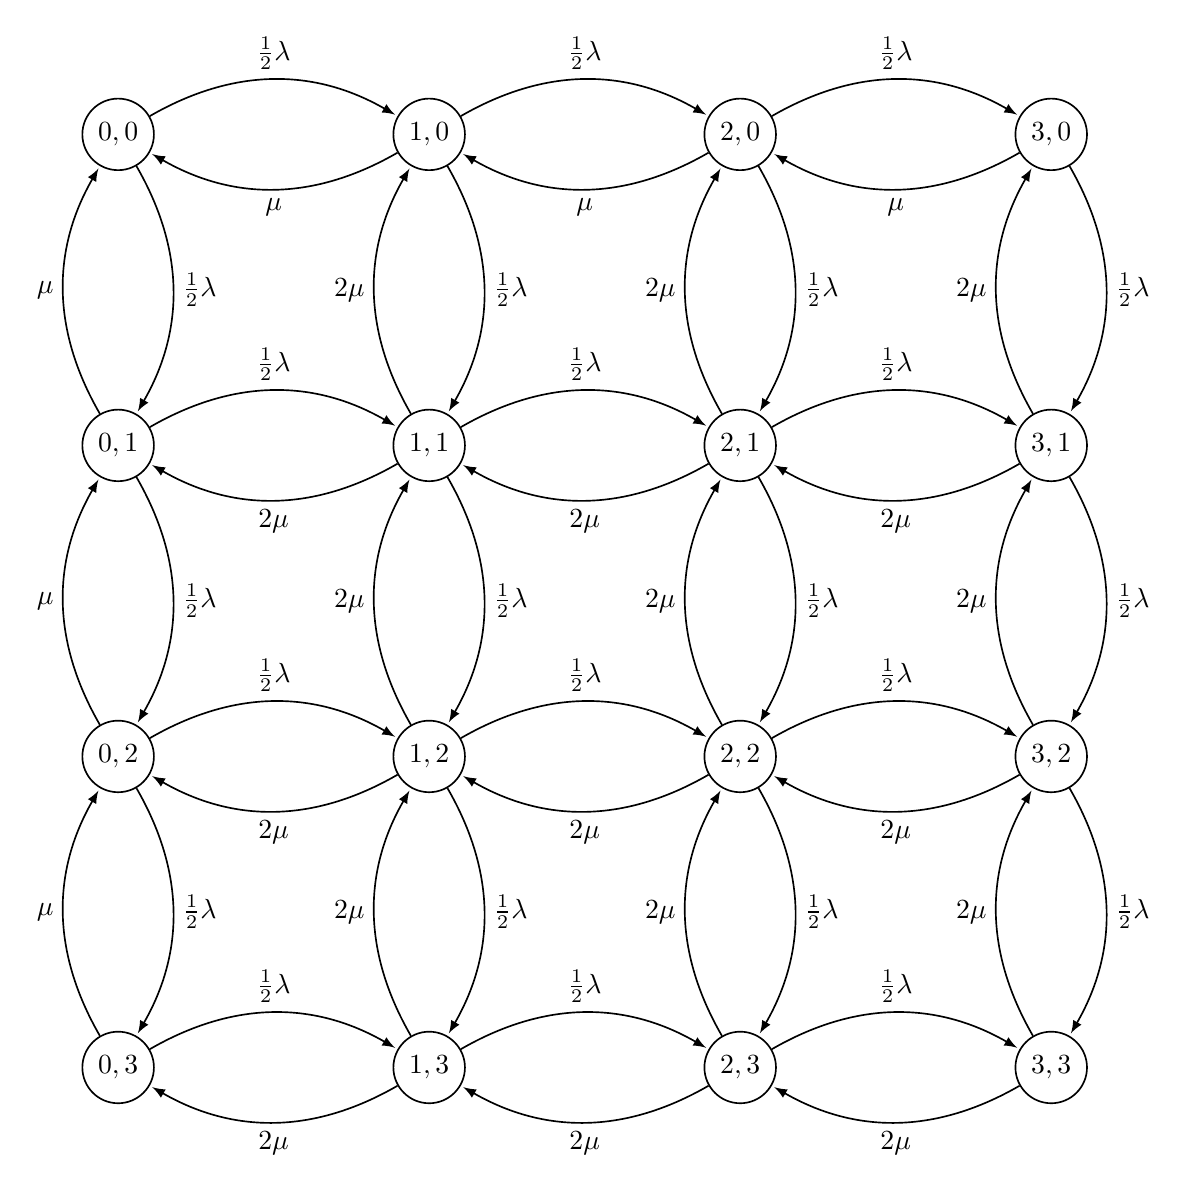
\begin{tikzpicture}[
            > = stealth, % arrow head style
            shorten > = 1pt, % don't touch arrow head to node
            auto,
            node distance = 3.95cm, % distance between nodes
            semithick % line style
        ]

	\node[state] (A) {$0,0$};
	\node[state] (B) [right of=A] {$1,0$};
	\node[state] (C) [right of=B] {$2,0$};
	\node[state] (D) [right of=C] {$3,0$};
	\node[state] (E) [below of=A] {$0,1$};
	\node[state] (F) [right of=E] {$1,1$};
	\node[state] (G) [right of=F] {$2,1$};
	\node[state] (H) [right of=G] {$3,1$};
	\node[state] (I) [below of=E] {$0,2$};
	\node[state] (J) [right of=I] {$1,2$};
	\node[state] (K) [right of=J] {$2,2$};
	\node[state] (L) [right of=K] {$3,2$};
	\node[state] (M) [below of=I] {$0,3$};
	\node[state] (N) [right of=M] {$1,3$};
	\node[state] (O) [right of=N] {$2,3$};
	\node[state] (P) [right of=O] {$3,3$};
	
 	\draw[-latex,bend left] (A) edge node {$\frac{1}{2}\lambda$} (B);
	\draw[-latex,bend left] (B) edge node {$\mu$} (A);
	\draw[-latex,bend left] (B) edge node {$\frac{1}{2}\lambda$} (C);
	\draw[-latex,bend left] (C) edge node {$\mu$} (B);
	\draw[-latex,bend left] (C) edge node {$\frac{1}{2}\lambda$} (D);
	\draw[-latex,bend left] (D) edge node {$\mu$} (C);
	
	\draw[-latex,bend left] (A) edge node {$\frac{1}{2}\lambda$} (E);
	\draw[-latex,bend left] (E) edge node {$\mu$} (A);
	\draw[-latex,bend left] (B) edge node {$\frac{1}{2}\lambda$} (F);
	\draw[-latex,bend left] (F) edge node {$2\mu$} (B);
	\draw[-latex,bend left] (C) edge node {$\frac{1}{2}\lambda$} (G);
	\draw[-latex,bend left] (G) edge node {$2\mu$} (C);
	\draw[-latex,bend left] (D) edge node {$\frac{1}{2}\lambda$} (H);
	\draw[-latex,bend left] (H) edge node {$2\mu$} (D);
	
	\draw[-latex,bend left] (E) edge node {$\frac{1}{2}\lambda$} (F);
	\draw[-latex,bend left] (F) edge node {$2\mu$} (E);
	\draw[-latex,bend left] (F) edge node {$\frac{1}{2}\lambda$} (G);
	\draw[-latex,bend left] (G) edge node {$2\mu$} (F);
	\draw[-latex,bend left] (G) edge node {$\frac{1}{2}\lambda$} (H);
	\draw[-latex,bend left] (H) edge node {$2\mu$} (G);
	
	\draw[-latex,bend left] (E) edge node {$\frac{1}{2}\lambda$} (I);
	\draw[-latex,bend left] (I) edge node {$\mu$} (E);
	\draw[-latex,bend left] (F) edge node {$\frac{1}{2}\lambda$} (J);
	\draw[-latex,bend left] (J) edge node {$2\mu$} (F);
	\draw[-latex,bend left] (G) edge node {$\frac{1}{2}\lambda$} (K);
	\draw[-latex,bend left] (K) edge node {$2\mu$} (G);
	\draw[-latex,bend left] (H) edge node {$\frac{1}{2}\lambda$} (L);
	\draw[-latex,bend left] (L) edge node {$2\mu$} (H);
	
	\draw[-latex,bend left] (I) edge node {$\frac{1}{2}\lambda$} (J);
	\draw[-latex,bend left] (J) edge node {$2\mu$} (I);
	\draw[-latex,bend left] (J) edge node {$\frac{1}{2}\lambda$} (K);
	\draw[-latex,bend left] (K) edge node {$2\mu$} (J);
	\draw[-latex,bend left] (K) edge node {$\frac{1}{2}\lambda$} (L);
	\draw[-latex,bend left] (L) edge node {$2\mu$} (K);
	
	\draw[-latex,bend left] (I) edge node {$\frac{1}{2}\lambda$} (M);
	\draw[-latex,bend left] (M) edge node {$\mu$} (I);
	\draw[-latex,bend left] (J) edge node {$\frac{1}{2}\lambda$} (N);
	\draw[-latex,bend left] (N) edge node {$2\mu$} (J);
	\draw[-latex,bend left] (K) edge node {$\frac{1}{2}\lambda$} (O);
	\draw[-latex,bend left] (O) edge node {$2\mu$} (K);
	\draw[-latex,bend left] (L) edge node {$\frac{1}{2}\lambda$} (P);
	\draw[-latex,bend left] (P) edge node {$2\mu$} (L);
	
	\draw[-latex,bend left] (M) edge node {$\frac{1}{2}\lambda$} (N);
	\draw[-latex,bend left] (N) edge node {$2\mu$} (M);
	\draw[-latex,bend left] (N) edge node {$\frac{1}{2}\lambda$} (O);
	\draw[-latex,bend left] (O) edge node {$2\mu$} (N);
	\draw[-latex,bend left] (O) edge node {$\frac{1}{2}\lambda$} (P);
	\draw[-latex,bend left] (P) edge node {$2\mu$} (O);
\end{tikzpicture}
\captionof{figure}{Cha\^ine de Markov pour des files de longueur inf\'erieures \`a 3}
\end{center}

C'est un processus Markovien car on n'a pas besoin de conna\^itre $N$ pour trouver $N+1$. 
On peut calculer les probabilit\'es suivantes :

\begin{align*}
\text{Probabilit\'e d'une arriv\'ee dans la file : } P(N_{1}(t+dt)=j+1 / N_{1}(t)=j)=\frac{1}{2}\lambda dt + o(dt) \\
\text{Probabilit\'e d'un d\'epart de file : } P(N_{1}(t+dt)=j-1 / N_{1}(t)=j)=\mu dt + o(dt)
\end{align*}

\newpage

\section*{File avec arriv\'ees d\'ecourag\'ees}

\newpage

\section*{Unit\'e de transmission de paquets}

\end{document}
